\chapter{Proposed method}


The main objective of this thesis is to perform a comprehensive comparison of different methods for time series classification, especially those dealing with missing data.
To achieve this goal, we have implemented several machine learning models and evaluated their effectiveness on a comprehensive dataset of satellite image time series.
The comparison and evaluation of these models will help to determine the most effective approach to handle missing data and improve the accuracy of time series classification tasks.


\section{Data preparation}

To ensure a comprehensive and unbiased comparison, the same dataset and evaluation metrics were used for all machine learning models in this thesis. 
Specifically, the dataset of choice was the Satellite Image Time Series (SITS) dataset, which contains a total of 137,606 time series of satellite images covering natural and semi-natural areas. 
Since the data available for this task is relatively limited, k-fold cross validation with $k=5$ and varying seeds was implemented to ensure that the results were not affected by the partitioning of the dataset. Additionally, to ensure a balanced distribution of classes within each fold, the dataset was partitioned into training/validation/test sets with equal representation of each class. 
To avoid spatial correlation, the same polygon pixels were not placed in the same sets.

The distribution of polygons and pixels for each class in the training, validation, and test sets can be observed in Table \ref{tab:dataset-splits}.
The splitting was done in a ratio of 60:20:20 for the training, validation, and test sets respectively, and no spatial correlation was taken into account during the partitioning process.
The table provides a comprehensive summary of the number of polygons and pixels for each class in each of the sets.

\begin{table}[H]
  \begin{tabular}{crrlcrrlcrrl}
     \cline{2-4} \cline{6-8} \cline{10-12} \\[-0.2cm]
          & \multicolumn{3}{c}{Train}                                 & \multicolumn{1}{l}{} & \multicolumn{3}{c}{Validation}                            & \multicolumn{1}{c}{} & \multicolumn{3}{c}{Test} \\[0.1cm]
    Class & Pol.                    & Pix.                      & \%  &                      & Pol.                    & Pix.  & \%                      &                      & Pol.   & Pix.    & \%    \\[0.2cm] \cline{2-4} \cline{6-8} \cline{10-12} \\[-0.2cm]
    1     & 427                     & 6486                      & 7   &                      & 142                     & 2266  & 8                       &                      & 143    & 1660    & 6     \\
    2     & 196                     & 3369                      & 3   &                      & 65                      & 803   & 3                       &                      & 67     & 993     & 3     \\
    3     & 49                      & 21298                     & 24  &                      & 16                      & 5308  & 20                      &                      & 17     & 5489    & 21    \\
    4     & 103                     & 30631                     & 35  &                      & 34                      & 8194  & 31                      &                      & 35     & 10350   & 40    \\
    5     & 133                     & 16933                     & 19  &                      & 44                      & 6362  & 24                      &                      & 46     & 5372    & 20    \\
    6     & 19                      & 1428                      & 1   &                      & 6                       & 309   & 1                       &                      & 7      & 338     & 1     \\
    7     & 23                      & 3399                      & 3   &                      & 7                       & 948   & 3                       &                      & 9      & 858     & 3     \\
    8     & 33                      & 2595                      & 3   &                      & 11                      & 1455  & 5                       &                      & 12     & 762     & 2     \\[0.2cm]\hline \\[-0.2cm]
    Tot   & \multicolumn{1}{l}{983} & \multicolumn{1}{l}{86139} & 100 & \multicolumn{1}{l}{} & \multicolumn{1}{l}{325} & 25645 & \multicolumn{1}{l}{100} & \multicolumn{1}{l}{} & 336    & 25822   & 100       
  \end{tabular}
  \caption{Distribution of classes, polygons and pixels for each dataset.}
  \label{tab:dataset-splits}
\end{table}

\section{Models}
To begin the process of selecting the most promising models for time series classification, the research began with a comprehensive review of the current state of the art in the field. This included a thorough investigation of published research studies and academic papers relevant to the research question. 
After analyzing and comparing the different approaches presented in the literature, the most promising models were selected for further investigation and testing.

Following the model selection phase, the research continued by studying the papers in depth and examining any available source code.
This process allowed us to gain a better understanding of the underlying algorithms and techniques used in each model, as well as any implementation details that might be relevant for adapting to the specific research needs.
Once the code was examined, it was adapted or implemented to meet our needs, and the performance of each model was evaluated on our dataset.

With the exception of the transformer models, which were implemented using PyTorch \cite{NEURIPS2019_9015}, all other models in this study were implemented using TensorFlow \cite{tensorflow2015-whitepaper}.
TensorFlow is a popular and widely used open source machine learning framework developed by Google, which provides an efficient and flexible way to build and train neural networks.
PyTorch, on the other hand, is another popular open-source machine learning framework developed by Facebook that provides dynamic computational graphs and a more python-like way to build and train neural networks, making it particularly suitable for research purposes.

Using both TensorFlow and PyTorch to implement the models was a challenging task, but it provided an opportunity to improve my skills in working with different deep learning frameworks.

To optimize the performance of each model, we conducted a thorough exploration of the hyperparameter space, varying various parameters such as learning rate, batch size, number of layers, number of units per layer, activation functions, regularization techniques, and others.
In addition, based on the results reported by the authors of each model, we also experimented with modifications to the architecture of the network, such as adding new layers, changing the order of the layers, or adjusting the size of the filters in the convolutional layers.

This process of hyperparameter tuning and model modification allowed us to identify the optimal settings for each model on our specific dataset, resulting in the best possible performance in terms of accuracy.
It is worth noting that this process was not always straightforward, and in some cases we encountered challenges such as overfitting, convergence problems, or long training times.
However, we were able to overcome these obstacles through careful experimentation and iteration.

During our experiments, we explored different methods to handle missing data in time series classification. 
To fully understand the impact of missing values on the performance of our models, we implemented two different approaches.
The first method involved replacing the missing values with zeros, while the second method involved using pre-imputed values based on linear multi-temporal interpolation \cite{IENCO201911}, which used the available cloud masks to fill the gaps in the time series data. 
By implementing both methods, we were able to compare the performance of the models in handling missing data in different ways.


\section{Weights and Biases}

Weights and Biases (W\&B) \cite{wandb} is a machine learning experiment tracking platform that allows users to log and compare the results of different experiments. 
In our research, we used W\&B to track experiments and compare the results of different models.

W\&B provides an intuitive experiment tracking interface that allows users to easily organize and compare results from different runs.
It also provides useful features such as visualization tools, automatic logging of metrics and hyperparameters, and integration with popular machine learning frameworks such as TensorFlow and PyTorch.

We used W\&B to log metrics and hyperparameters such as accuracy, learning rate, batch size, and more. 
This allowed us to easily compare the results of different models and identify which hyperparameters had the most significant impact on performance.

In addition to logging metrics and hyperparameters, W\&B also allowed us to visualize the results in a variety of ways. 
We used the platform's dashboard to plot and compare the different metrics across experiments.

\begin{figure}[H]
  \centering
  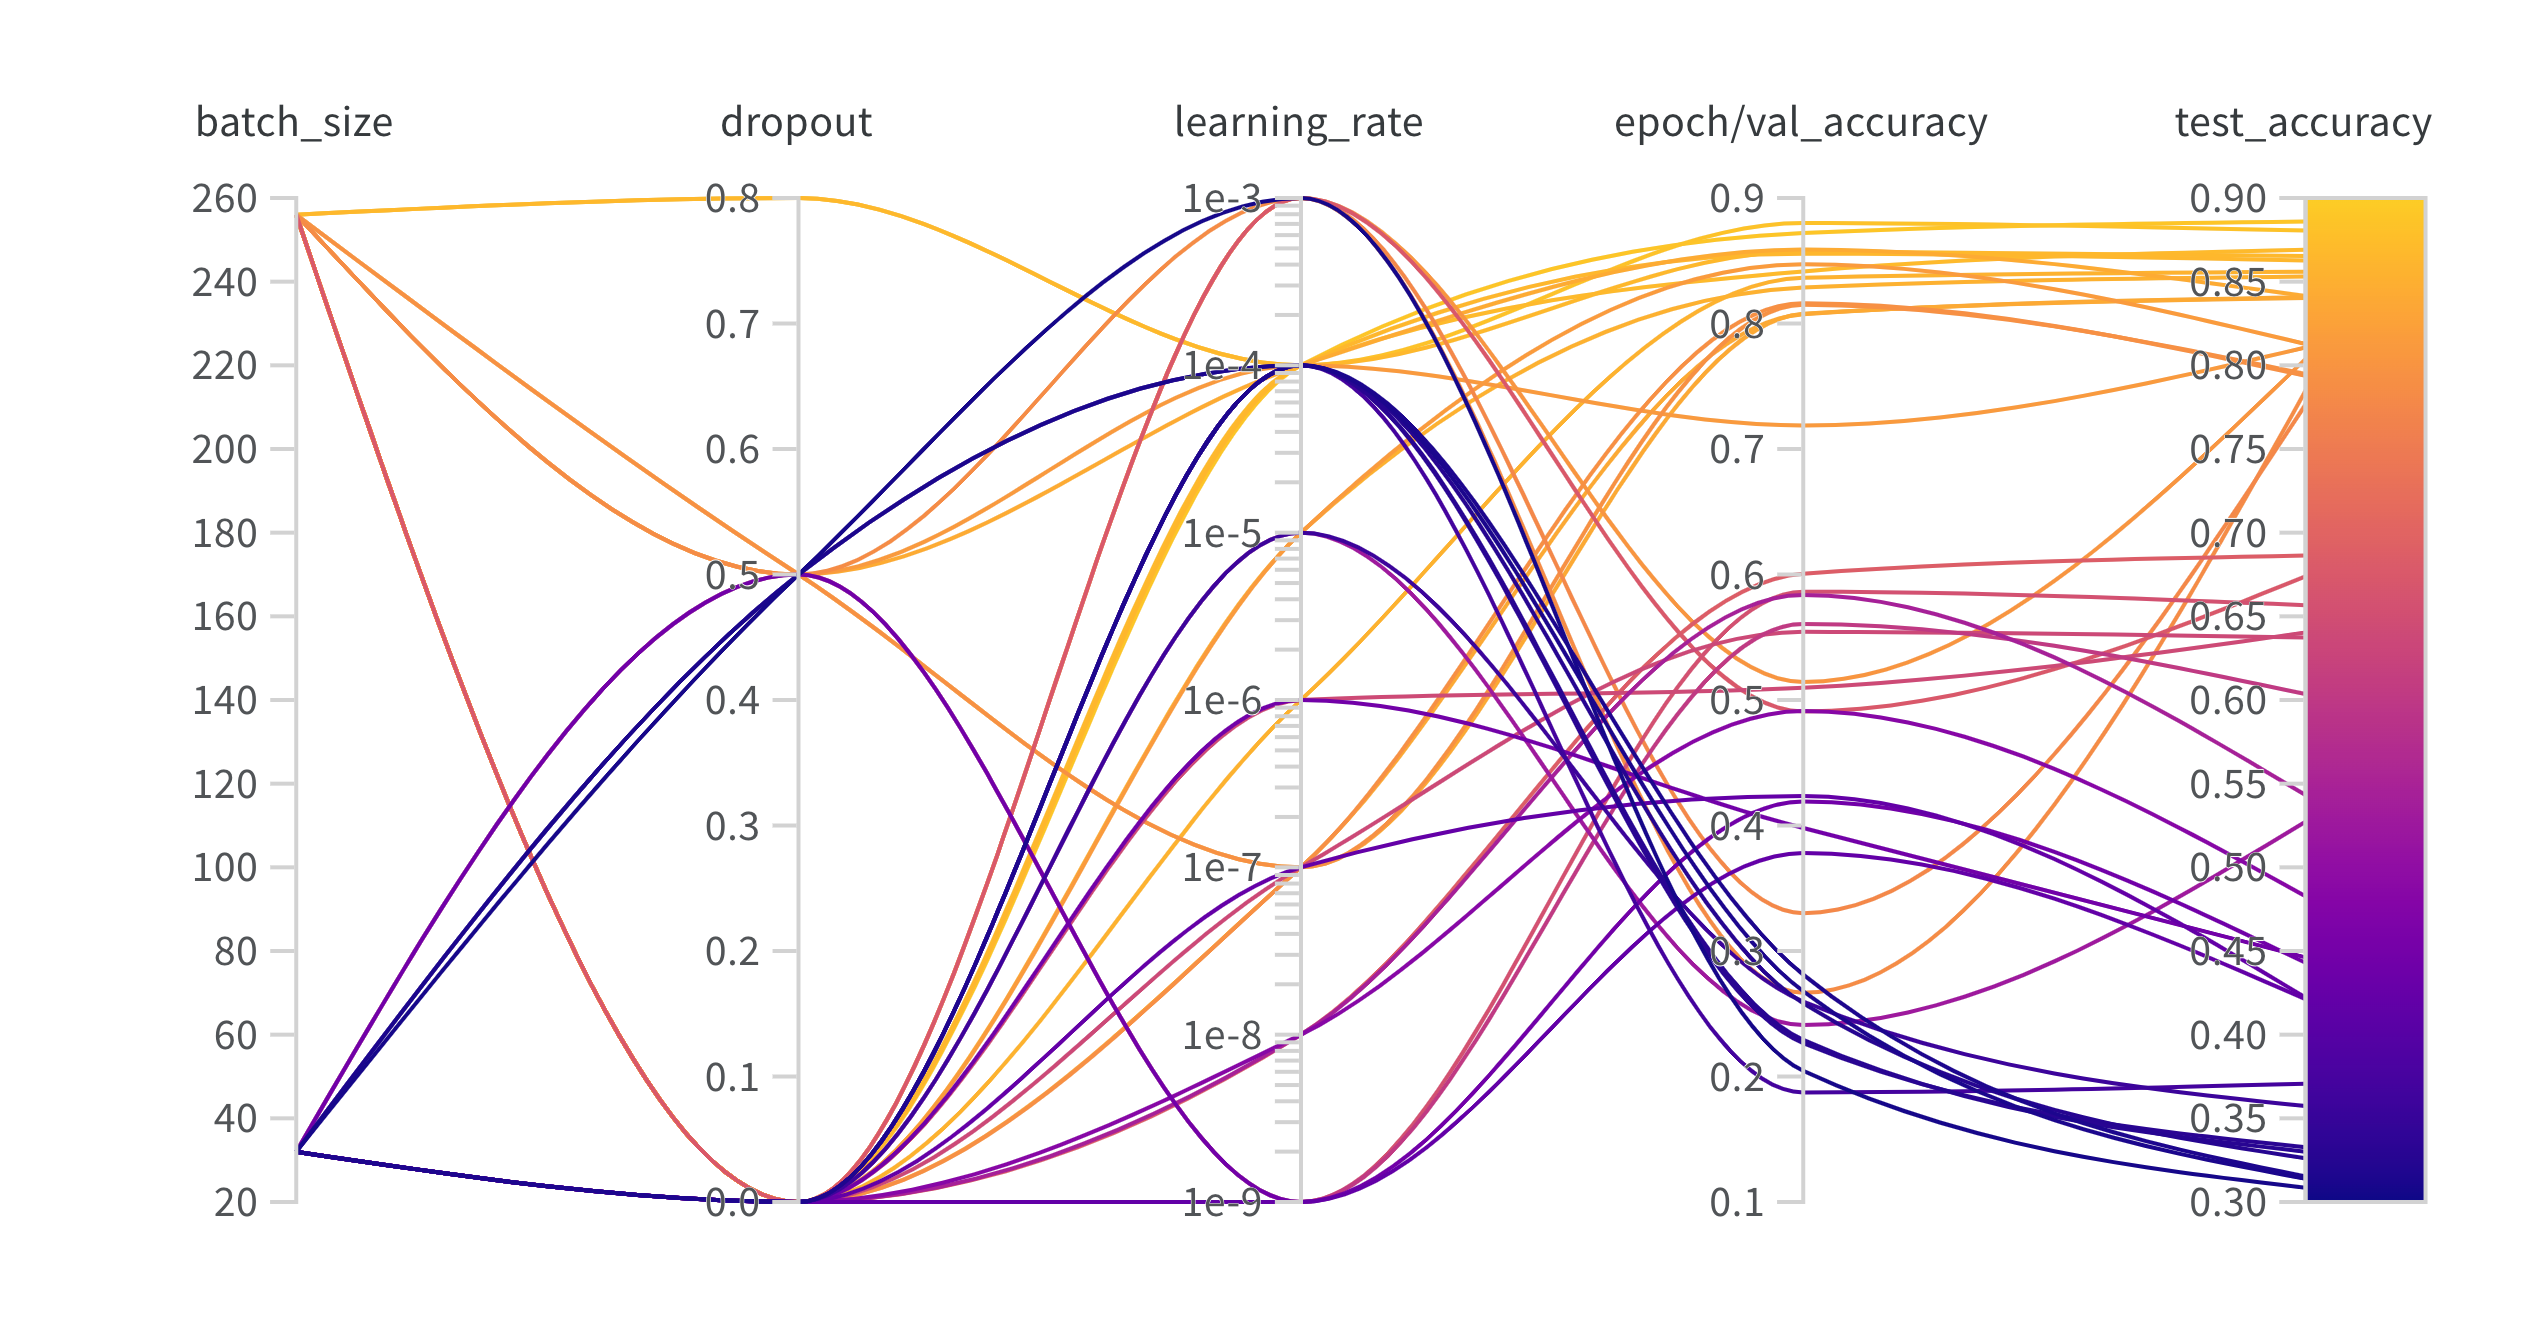
\includegraphics[width=0.4\textwidth]{wandb1}
  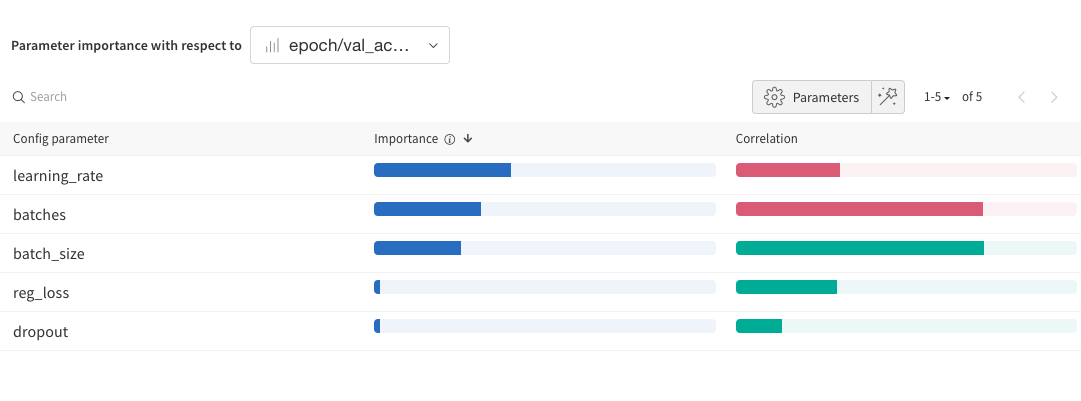
\includegraphics[width=0.4\textwidth]{wandb2}
  \caption{W\&B panels showing parallel coordinates plot of hyperparameters and metrics on the left, and parameter importance plot on the right.}
\end{figure}


To facilitate hyperparameter tuning, W\&B provides a powerful tool called Sweeps.
This feature allows an efficient and automated search of the hyperparameter space, where the user defines a range of values for each hyperparameter and W\&B does the rest.
You can add multiple agents to run the sweeps in parallel, which can significantly reduce the time required to complete the search.
In addition, the results of the sweeps can be easily visualized and compared, providing valuable insight into the impact of different hyperparameters on the performance of the model.

\begin{figure}[H]
\begin{lstlisting}[language=yaml]
method: random
metric:
  goal: maximize
  name: epoch/val_accuracy
parameters:
  G_epoch:
    value: 1
  batch_size:
    value: 32

  # ... more hyperparameters

  hidden_size:
    value: 128
  learning_rate:
    values:
      - 1e-05
      - 1e-06
      - 1e-07
      - 1e-08
      - 1e-09
program: train.py
\end{lstlisting}
\caption{Example of Sweep configuration}
\end{figure}

Overall, W\&B proved to be an essential tool for our project, allowing us to keep track of the experiments and compare the results of the different models. 
Its intuitive interface and powerful visualization tools made it easy to use and allowed us to quickly gain insight into the performance of the models.




